\documentclass[10pt,twocolumn,letterpaper]{article}

\usepackage{cvpr}
\usepackage{times}
\usepackage{epsfig}
\usepackage{graphicx}
\usepackage{amsmath}
\usepackage{amssymb}

% Include other packages here, before hyperref.

% If you comment hyperref and then uncomment it, you should delete
% egpaper.aux before re-running latex.  (Or just hit 'q' on the first latex
% run, let it finish, and you should be clear).
\usepackage[pagebackref=true,breaklinks=true,letterpaper=true,colorlinks,bookmarks=false]{hyperref}

% \cvprfinalcopy % *** Uncomment this line for the final submission

\def\cvprPaperID{****} % *** Enter the CVPR Paper ID here
\def\httilde{\mbox{\tt\raisebox{-.5ex}{\symbol{126}}}}

% Pages are numbered in submission mode, and unnumbered in camera-ready
\ifcvprfinal\pagestyle{empty}\fi
\begin{document}

%%%%%%%%% TITLE
\title{Efficient Visual Saliency detection with Deep Learning}

\author{First Author\\
Institution1\\
Institution1 address\\
{\tt\small firstauthor@i1.org}
% For a paper whose authors are all at the same institution,
% omit the following lines up until the closing ``}''.
% Additional authors and addresses can be added with ``\and'',
% just like the second author.
% To save space, use either the email address or home page, not both
\and
Second Author\\
Institution2\\
First line of institution2 address\\
{\tt\small secondauthor@i2.org}
}

\maketitle
%\thispagestyle{empty}

%%%%%%%%% ABSTRACT
\begin{abstract}
Visual saliency is an important component of attention.
It helps animals survive and can also be used by computer vision applications
to filter out irrelevant information from high volumes of data.
In this work, we present a new fully convolutional neural network
architecture designed for detecting visual saliency,
with architecture and data pre-processing methods specific
for the task of visual saliency detection.
Experiments carried out with the MIT300 benchmark presented state-of-the-art
performance and a parameter reduction of 3/4 compared to similar models.
\end{abstract}

%%%%%%%%% BODY TEXT
\section{Introduction}
One of the most challenging unsolved problems in Artificial Intelligence
is vision.
However, it is fundamental for the conception of systems that interact
in the real physical world.
Such systems would be useful for applications in areas like
domestic services, industry, and agriculture,
with great potential for the benefit of society.

Vision is remarkable data and computationally intensive.
In humans, approximately half of the brain is involved in
vision-related tasks~\cite{fixott_1957}.
Even our minds cannot handle all the sheer amount of sensorial information
received every second. In order to deal with this amount of data,
humans have attentional systems, a fundamental mechanism
that, among other functions, filters out irrelevant information
-- either visual or from other senses-- and helps us focusing our cognitive
processes on what is important at a given moment.
These facts are a strong evidence that in order to help to solve
vision problems, attention should be applied.

Visual attention can be defined as the delimitation of a certain spatial
the region on an image for further cognitive processing~\cite{treisman_1980}.
The phenomenon emerges from two fundamentally different processes:
the \emph{top-down} mechanism that implements our longer-term cognitive
strategies by biasing attention according to one's interests
(e.g. find a red apple in a tree because of hunger,
which will make red be more recognizable on the scene),
and the \emph{bottom-up} mechanism~\cite{colombini_2016},
a process generated through external stimuli
that captures one's attention from its conspicuousness level.
In this work, we focus on the latter, also named visual saliency.

Visually salient regions on images are usually represented by
\emph{saliency maps} (Figure~\ref{fig:example}). In these maps, images are generated such that
areas with high-valued pixels express high saliency on the original image,
whereas regions with low-valued pixels represent low saliency.
Datasets with such maps are obtained by collecting eye-fixation
data from humans while observing the scenes.

\begin{center}
\begin{figure}[t]
\begin{tabular} {cc}
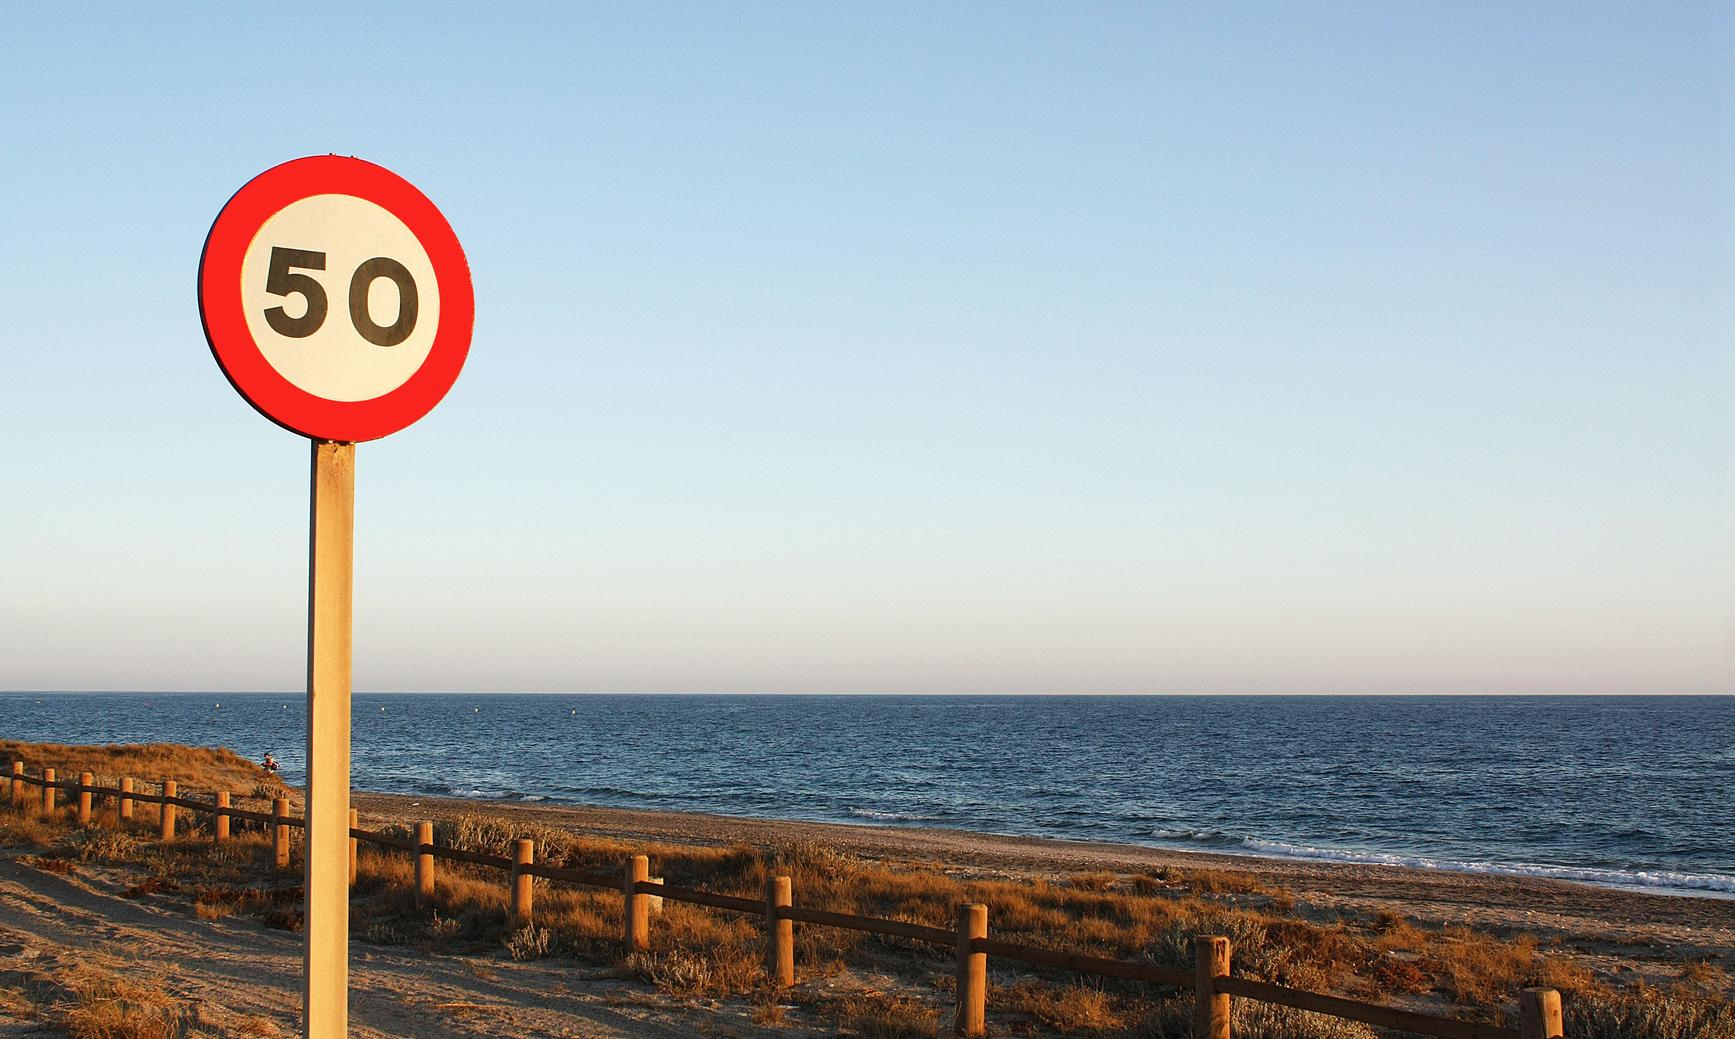
\includegraphics[width=0.22\textwidth]{./img/traffic_sign_s.jpg} &
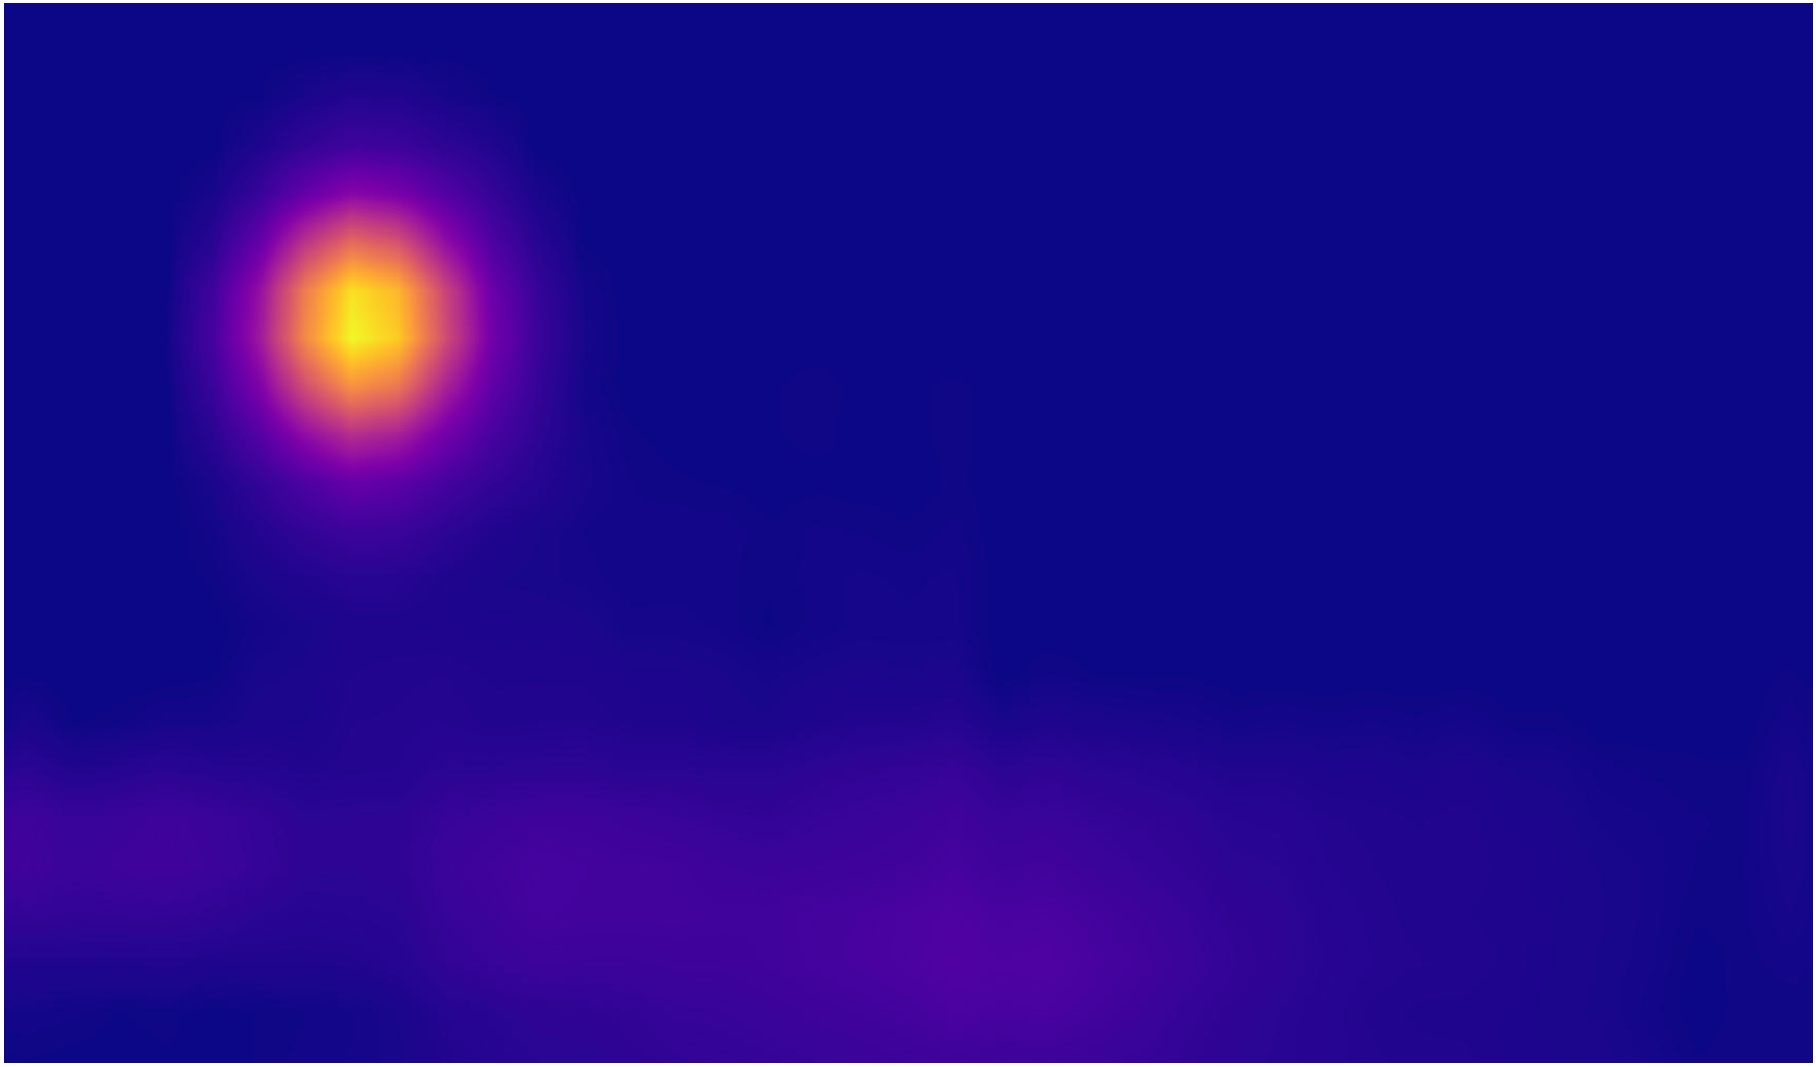
\includegraphics[width=0.22\textwidth]{./img/traffic_sign_m.jpg}\\
(a) & (b)
\end{tabular}
\caption{Example of visual saliency.
    b) is the saliency map where brighter pixels (warmer colors)
    represent regions more salient to humans on the original image a).}
\label{fig:example}
\end{figure}
\end{center}

\subsection{Related work}
Early computational models of visual saliency were generally built based on
filtering of images for extraction of a pre-selected set of features
considered important for \emph{bottom-up} attention.
\emph{Vocus}~\cite{frintrop_2005} is a computational model that extracts
features which are shown to be naturally salient to humans such as color/luminance
contrast and orientation from different scales of the image.

A rapid change of paradigm occurred around 2015 when \emph{Deep Learning}
techniques showed to be very effective in the generation of saliency
maps.
\emph{Salicon}~\cite{jiang_2015} demonstrated that the use of
convolutional neural networks with weights initialized from
image classification networks, e.g. \emph{VGG-16}~\cite{zisserman_2014}
could considerably increase the similarity of computed maps to those
generated from humans, whereas \emph{Salicon} uses different scales of the image as input to capture relevant
information in the context of saliency, using the same network weights
for each dimension.
\emph{ML-Net}~\cite{cornia_2016} uses the output of different layers
of \emph{VGG-16}, combining them in many dimensions and various levels of
abstraction.
\emph{DeepFix}~\cite{kruthiventi_2015} extends a pre-trained model with
inception~\cite{szegedy_2014} layers -- which use information from different
scales of the image -- and a component for center bias, a phenomenon that arises from our tendency to take pictures with relevant
objects at the center of the image.
\emph{Salnet}~\cite{pan_2016} explores two models: a shallow convolutional network followed by a fully-connected layer and a fully convolutional
neural network with first layers' weights initialized from \emph{VGG-16}.
Models that use weights from VGG-16 all use RGB images as input, subtracting
channel-wise the mean of the dataset for each RGB channel.

However, current state of the art models are in general quite expensive computationally,
partially because most of them are based on big pre-trained networks.
The convolutional layers of \emph{VGG-16} are composed of around 14.7
million parameters.
While pre-trained weights from classification tasks showed to be effective
for saliency prediction, it is reasonable to question whether
creating a proper network from scratch could yield a smaller amount of
parameters that are more efficient for the sole task of saliency prediction.
Also, there are some data processing methods from previous work on
psychology-based models that were not used in current models but
are considered worthwhile to explore,
such as using global information from the scene and a color space more
closely related to human vision.

In this context, this work aims at building a visual saliency model that is a) effective,
yielding results similar to another state of the art models,
and b) relatively simple and computationally efficient.
It is important that both criteria are matched in order to extend the
model in the future for video and real-time computer vision applications
such as navigating robots.

\section{Proposed model}
Figure~\ref{fig:model} shows the overall architecture of the fully
convolutional neural network proposed in this work.
It extracts features from increasingly smaller dimensions of the
input image.
The network is composed of four main blocks:

\begin{enumerate}
    \item The first level extracts low-level features from the input image, of
        dimensions $W\times H \times 3$ (width, height, depth), using
        a single layer with 48 convolution filters with ReLu activation
        followed by max-pooling that reduces the image by a factor of two.
        Experiments showed that by further decreasing the number of filters in this
        layer considerably hurts performance, which makes sense because it is
        important to capture high spatial frequency and high contrast
        information in the context of visual saliency.
    \item The second level extracts low-medium level features from the
        input of dimensions $W/2 \times H/2 \times 48$ using two layers
        with 64 and 96 convolution filters, respectively, followed by ReLU
        activation and max-pooling.
    \item The third level extracts medium-high level features from input with
        dimensions $W/4 \times H/4 \times 96$ using four convolution layers
        in sequence with 128, 128, 144 and 144 filters.
        Every convolution layer is followed by ReLu.
        Max-pooling is carried out at the end.
        A considerable depth in this level was found to be important for
        the network's performance.
    \item The fourth and last level is composed of eight inception blocks
        that extract high level features from the input with
        dimensions $W/8 \times H/8 \times 96$.
        Great level of depth and Inception blocks were found to be very
        important at this level.
        A $1 \times 1$ convolution makes a linear combination of the output
        maps at the end of the 8 inception blocks, followed by ReLu, producing
        the final saliency map of dimensions $W/8 \times H/8 \times 1$.
        The saliency map is then resized to the original dimensions using
        bicubic interpolation.
\end{enumerate}

\begin{figure*}
\begin{center}
\def\svgwidth{1.8\columnwidth}
\input{./img/model.pdf_tex}
\label{fig:model}
    \caption{Overview of the network.
        Filters sizes are in format width$\times$height\_stride.}
\end{center}
\end{figure*}

Figure \ref{fig:inception} illustrates the inception
architecture~\cite{szegedy_2014}
used in each block where filters of size $5 \times 5$, $3 \times 3$
(both preceded by $1\times 1$ convolutions in order to reduce the number
of input filters), $1 \times 1$, and a max-pooling of size $3 \times 3$ are applied.
Each of these operations is executed in parallel from the same input
and the outputs are concatenated at the output.
Inception allows the network to use
information from different spatial dimensions as well as previous
layers (lower level saliency information) in the final map
computation, which is considered to be important for visual saliency.
The network has a total of $3717841$ parameters, a very low number
compared to other models. Table \ref{table:inception} details the filter configuration for the inception layers.

\begin{figure}[!htb]
    \centering
    \def\svgwidth{\linewidth}
    \input{./img/inception.pdf_tex}
    \caption{Inception block layout.}
   \label{fig:inception}
\end{figure}

\begin{table*}
\centering
	\small
\label{table:inception}
\caption{Number of filters used in each inception block.}
\begin{tabular}{|c|c|c|c|c|c|c|}
	\hline
    Block & pool & conv 1$\times$1 & 3$\times$3 reduce &
    conv 3$\times$3 & 5$\times$5 reduce & conv 5$\times$5\\
    \hline
    1 & 96 & 128 & 96 & 192 & 48 & 96\\
    \hline
    2 & 64 & 128 & 80 & 160 & 24 & 48\\
    \hline
    3 & 64 & 128 & 80 & 160 & 24 & 48\\
    \hline
    4 & 64 & 128 & 96 & 192 & 28 & 56\\
    \hline
    5 & 64 & 128 & 96 & 192 & 28 & 56\\
    \hline
    6 & 64 & 128 & 112 & 224 & 32 & 64\\
    \hline
    7 & 64 & 128 & 112 & 224 & 32 & 64\\
    \hline
    8 & 112 & 160 & 128 & 256 & 40 & 80\\
    \hline
\end{tabular}
\end{table*}

\subsection{Data pre-processing}
Input images were resized to dimensions $320\times240\times3$.
Each image is normalized channel-wise by the subtraction of
the channel mean and division by the standard deviation:
$$C = \frac{C - \mu_C}{\sigma_C}$$
Most models used for comparison and cited in this work use RGB images
normalized channel-wise using statistics computed from the dataset.
However, visual saliency is highly connected to the context of the
image, hence saliency depends on the local context.

In our work, images are converted from RGB color space to the LAB color
space.
\emph{Vocus}~\cite{frintrop_2005} cites that the
LAB color space is more closely related to human vision once it encompasses
red-green, yellow-blue and
luminance maps.

\subsection{Implementation}
The network was implemented using \emph{Theano} \texttt{0.9.0.dev}
along with \emph{Lasagne} \texttt{0.2.dev1}
on a machine with \emph{Ubuntu 16.04 LTS} and
kernel \emph{Linux} \texttt{4.8.0-54-generic}.
Training was conducted on a GPU \emph{NVIDIA GTX 1080} and the
code is available at \texttt{https://goo.gl/5JZMjb}

\subsection{Training}
Two datasets were considered:
\emph{SALICON}~\cite{jiang_2015}, with 15000 images, and
\emph{Judd}~\cite{judd}, with 1003 images.
The network was trained using Stochastic Gradient Descent with Nesterov
Momentum of $0.9$.
\emph{SALICON} was first used with data augmentation by flipping images
horizontally and vertically and the target normalized by mean-std
(Last conv layer had ReLu removed in this step).
Mean-std normalization of targets was applied because it led to faster
convergence.

The loss function to be minimized was the \emph{Cross Correlation},
because it penalizes symmetrically false positives and false negatives.
A more detailed explanation of the metric is given in
section~\ref{sec:metrics}.
Training iterated for 5 epochs with learning rate of $0.009$
and then for 3 epochs with learning rate of $0.001$.
Then, unit normalization on targets started being used.
The network was trained for 1 epoch with learning rate of
$3\times10^{-5}$ and L2 regularization of $10^{-4}$. Finally, Judd dataset was used with data augmentation by flipping images horizontally and the target normalized by unit normalization.
Training iterated for 2 epochs with learning rate of
$5\times10^{-5}$ and L2 regularization of $3\times10^{-5}$. Batch sizes were 10 for SALICON and 2 for Judd. The complete training process took around two and a half hours.

\begin{figure*}
\begin{center}
    \begin{tabular} {ccc}
    Stimulus & Ground-truth & Proposed Model\\
    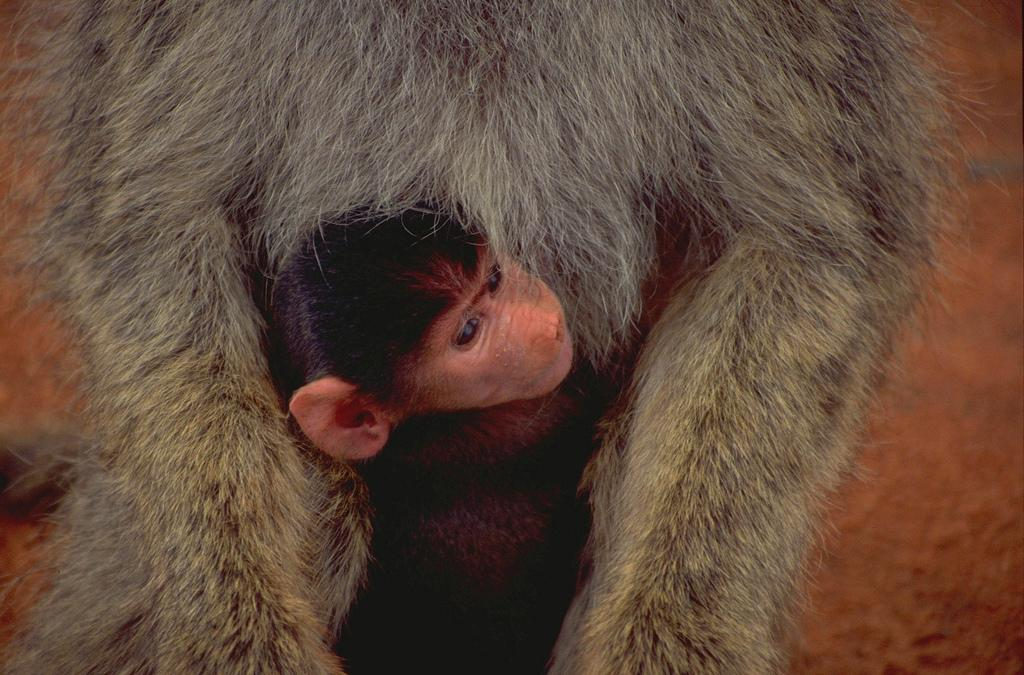
\includegraphics[width=0.25\textwidth]{./img/monkey_s.jpg} &
    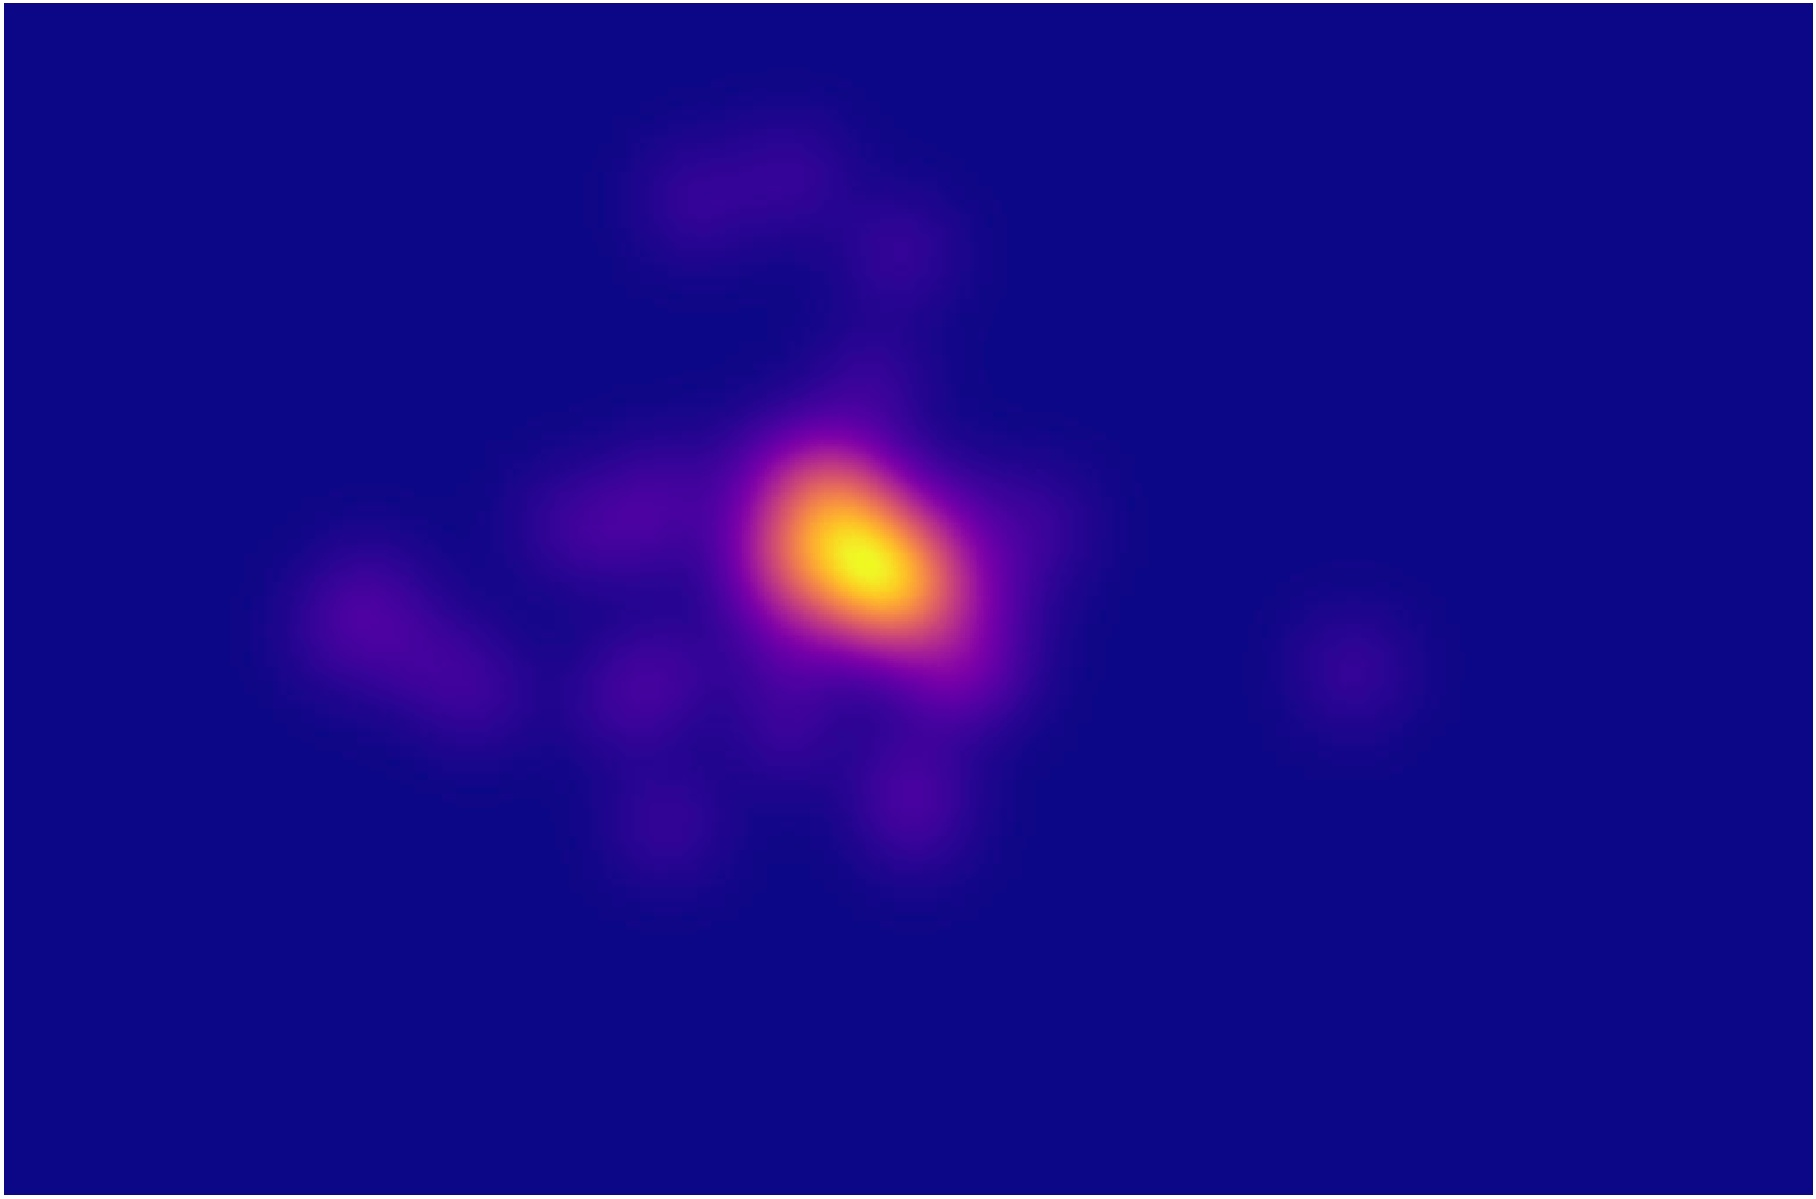
\includegraphics[width=0.25\textwidth]{./img/monkey_gt.jpg} &
    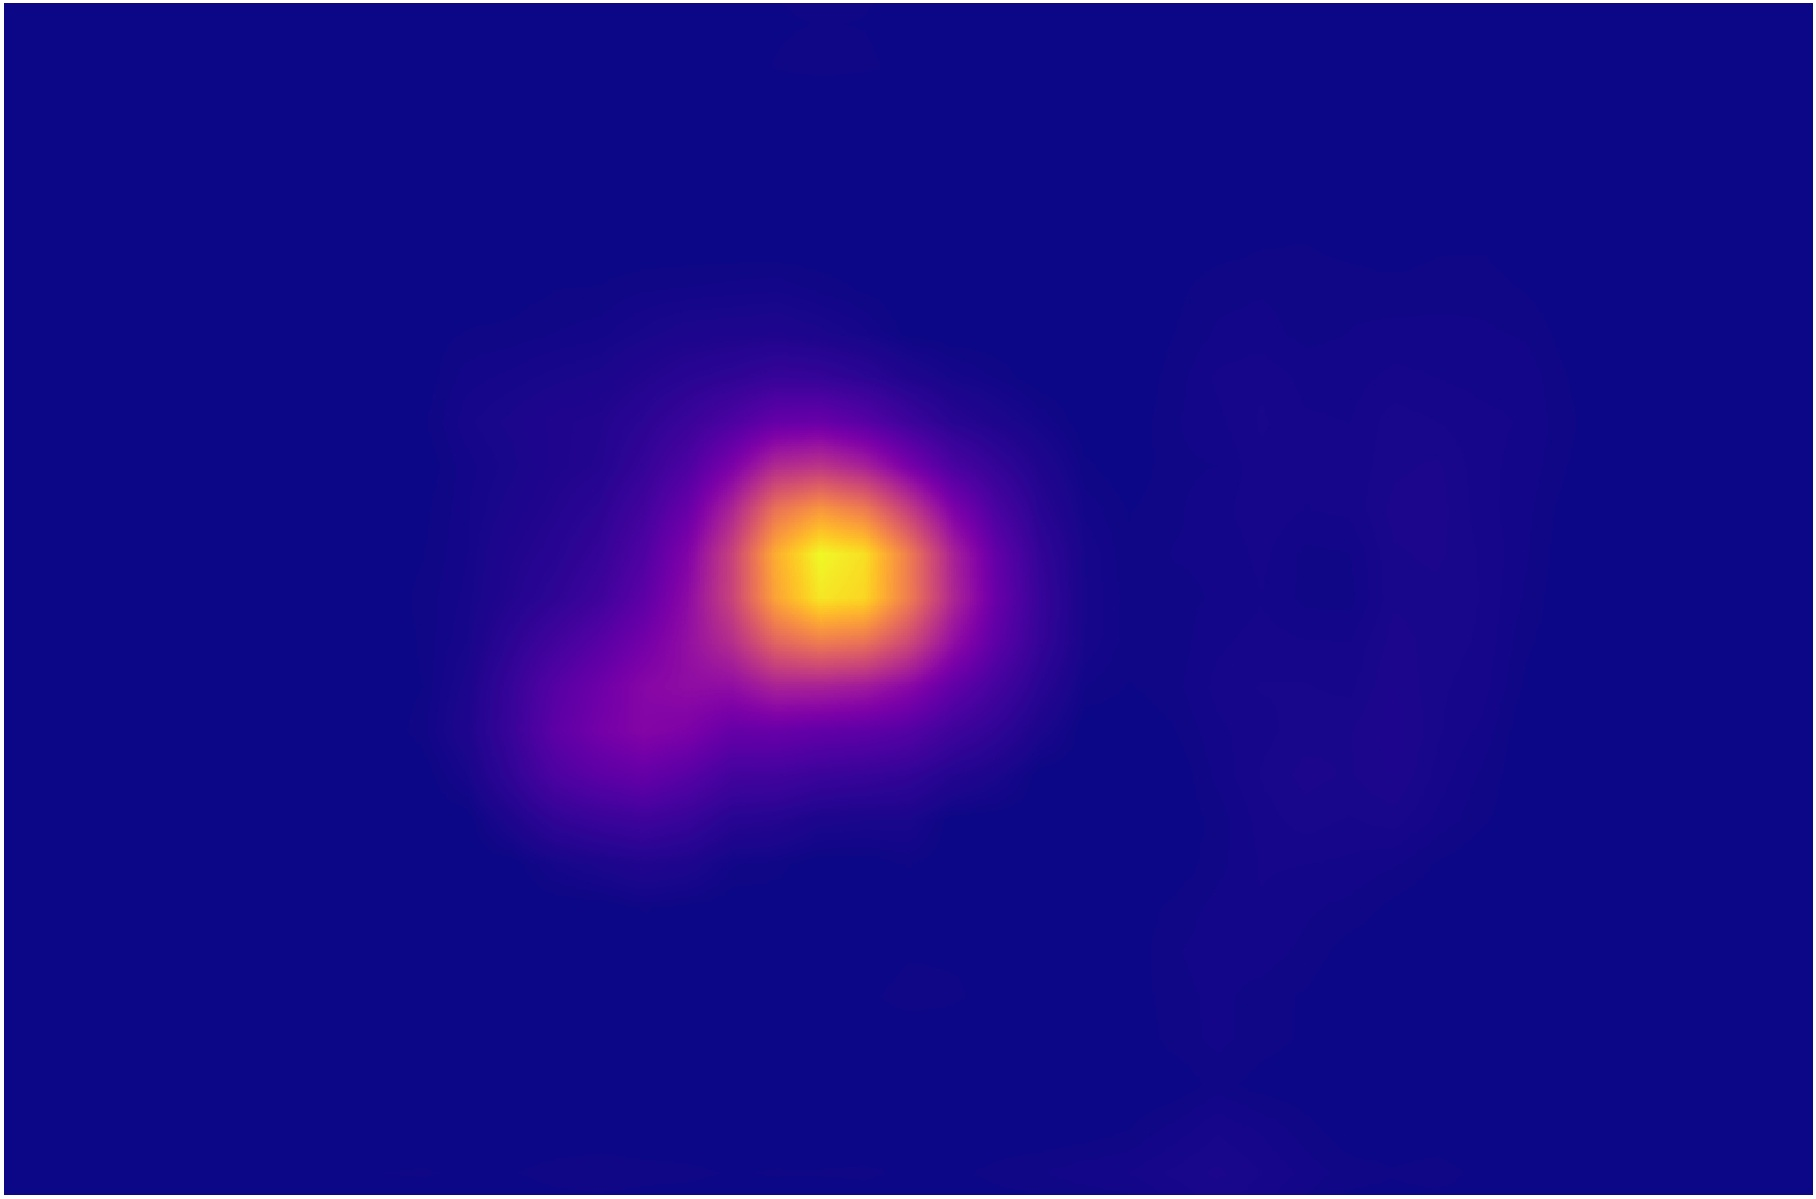
\includegraphics[width=0.25\textwidth]{./img/monkey_m.jpg}\\
    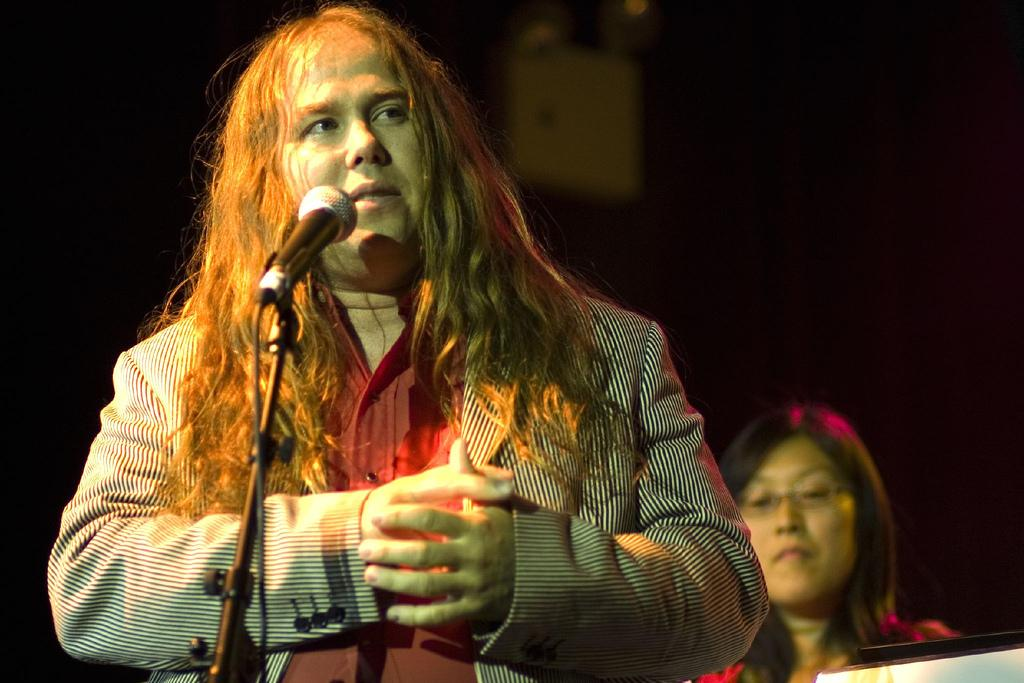
\includegraphics[width=0.25\textwidth]{./img/person_s.jpg} &
    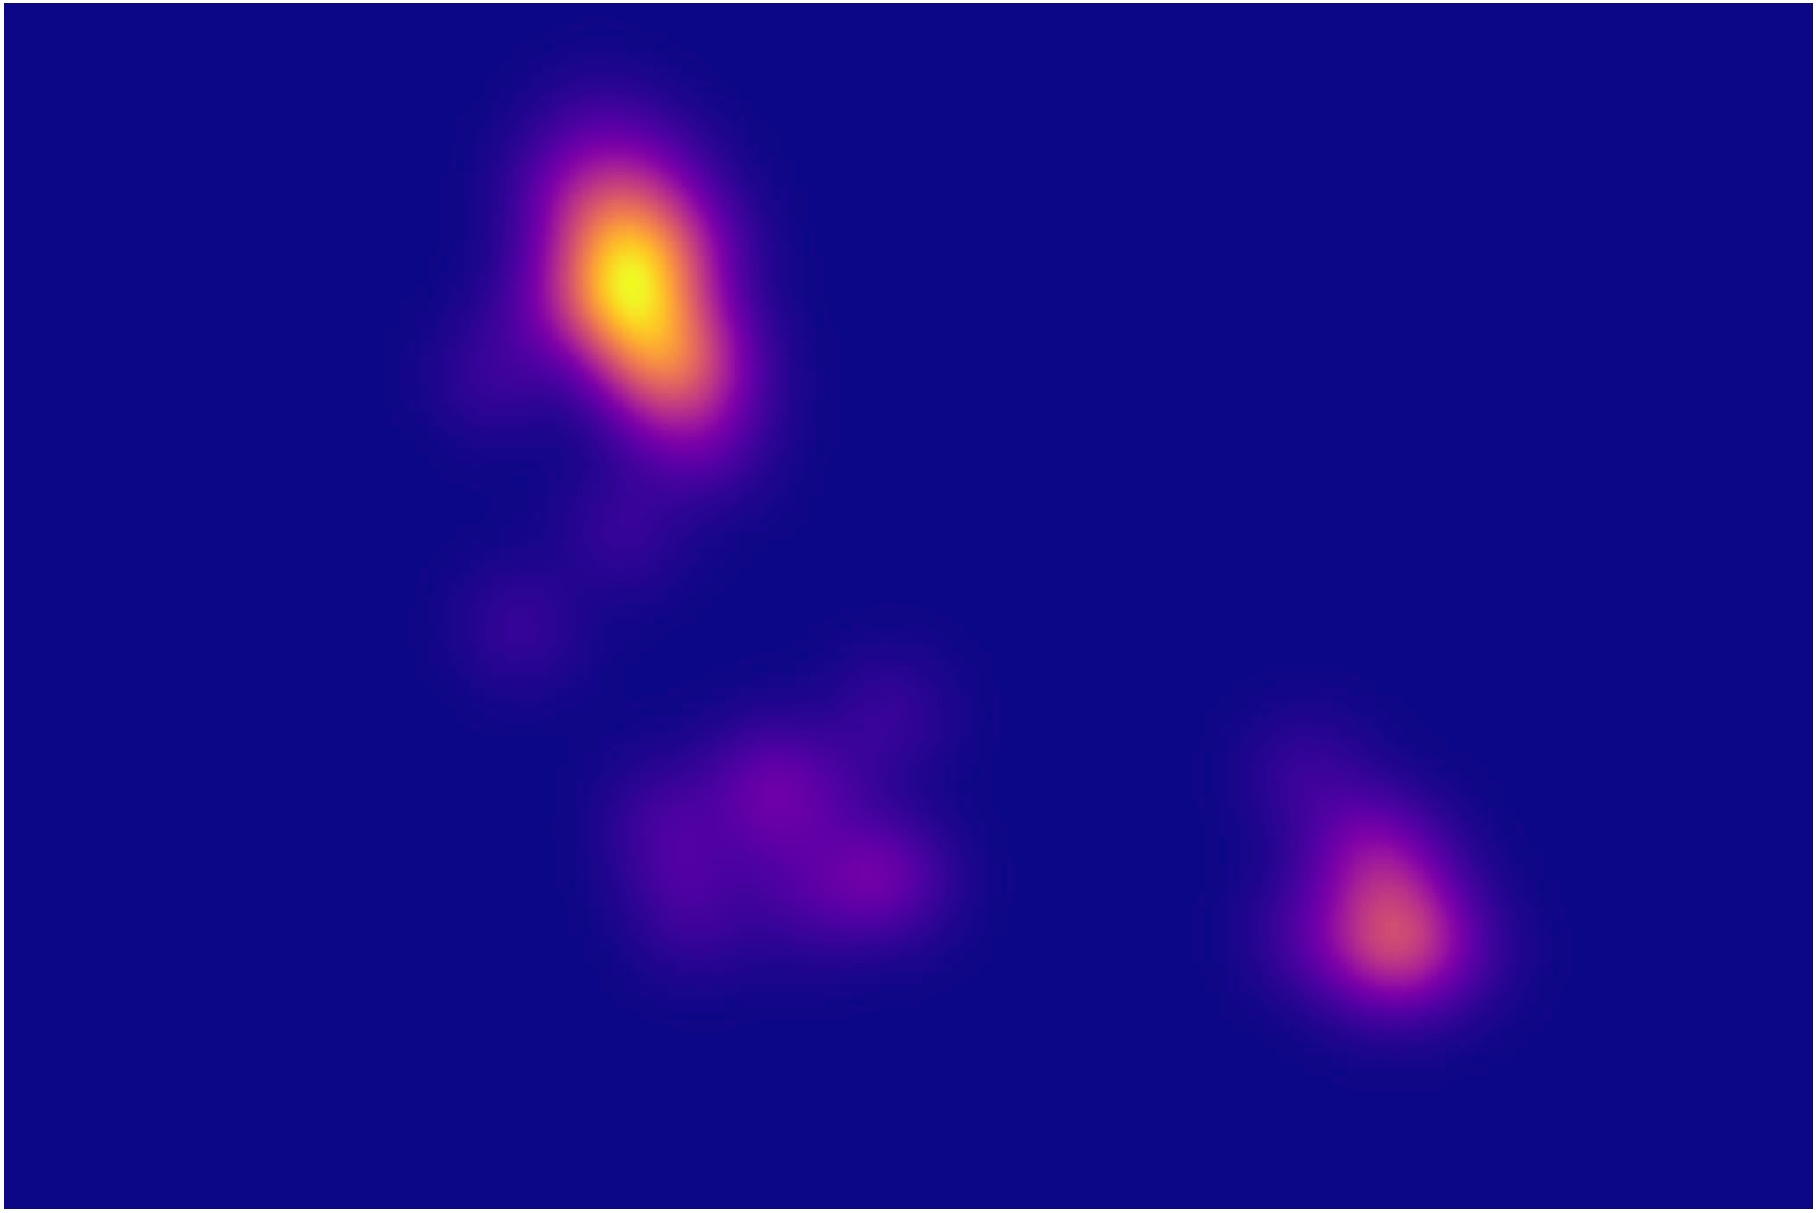
\includegraphics[width=0.25\textwidth]{./img/person_gt.jpg} &
    
\includegraphics[width=0.25\textwidth]{./img/person_m.jpg}\\
    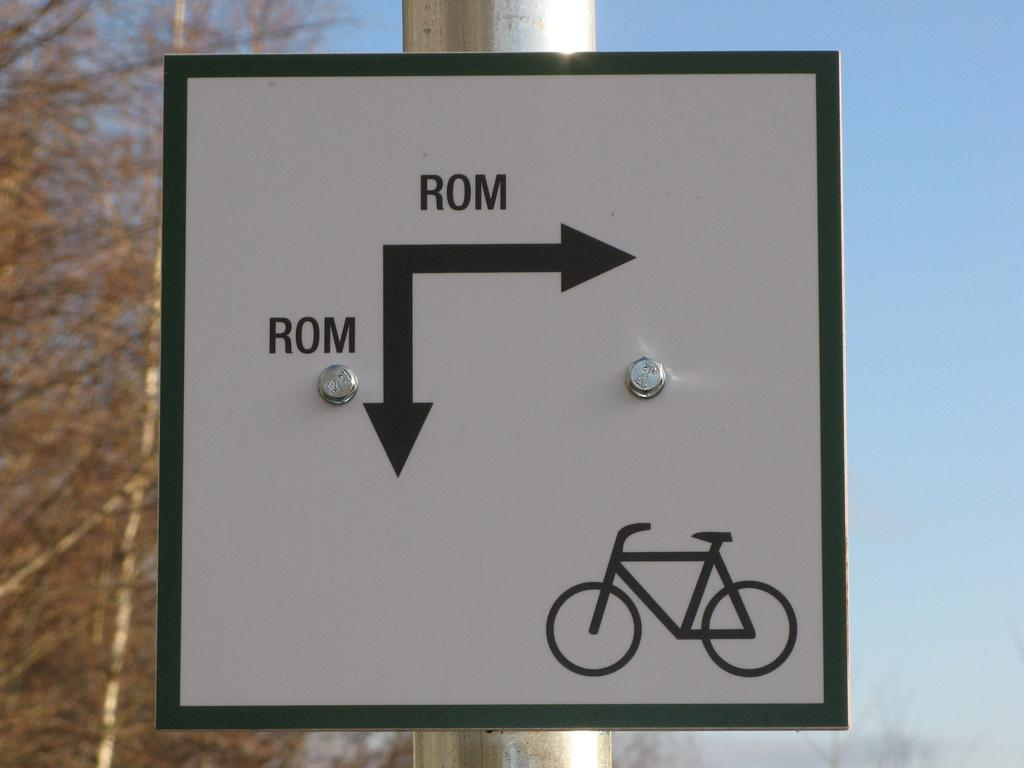
\includegraphics[width=0.25\textwidth]{./img/sign_s.jpg} &
    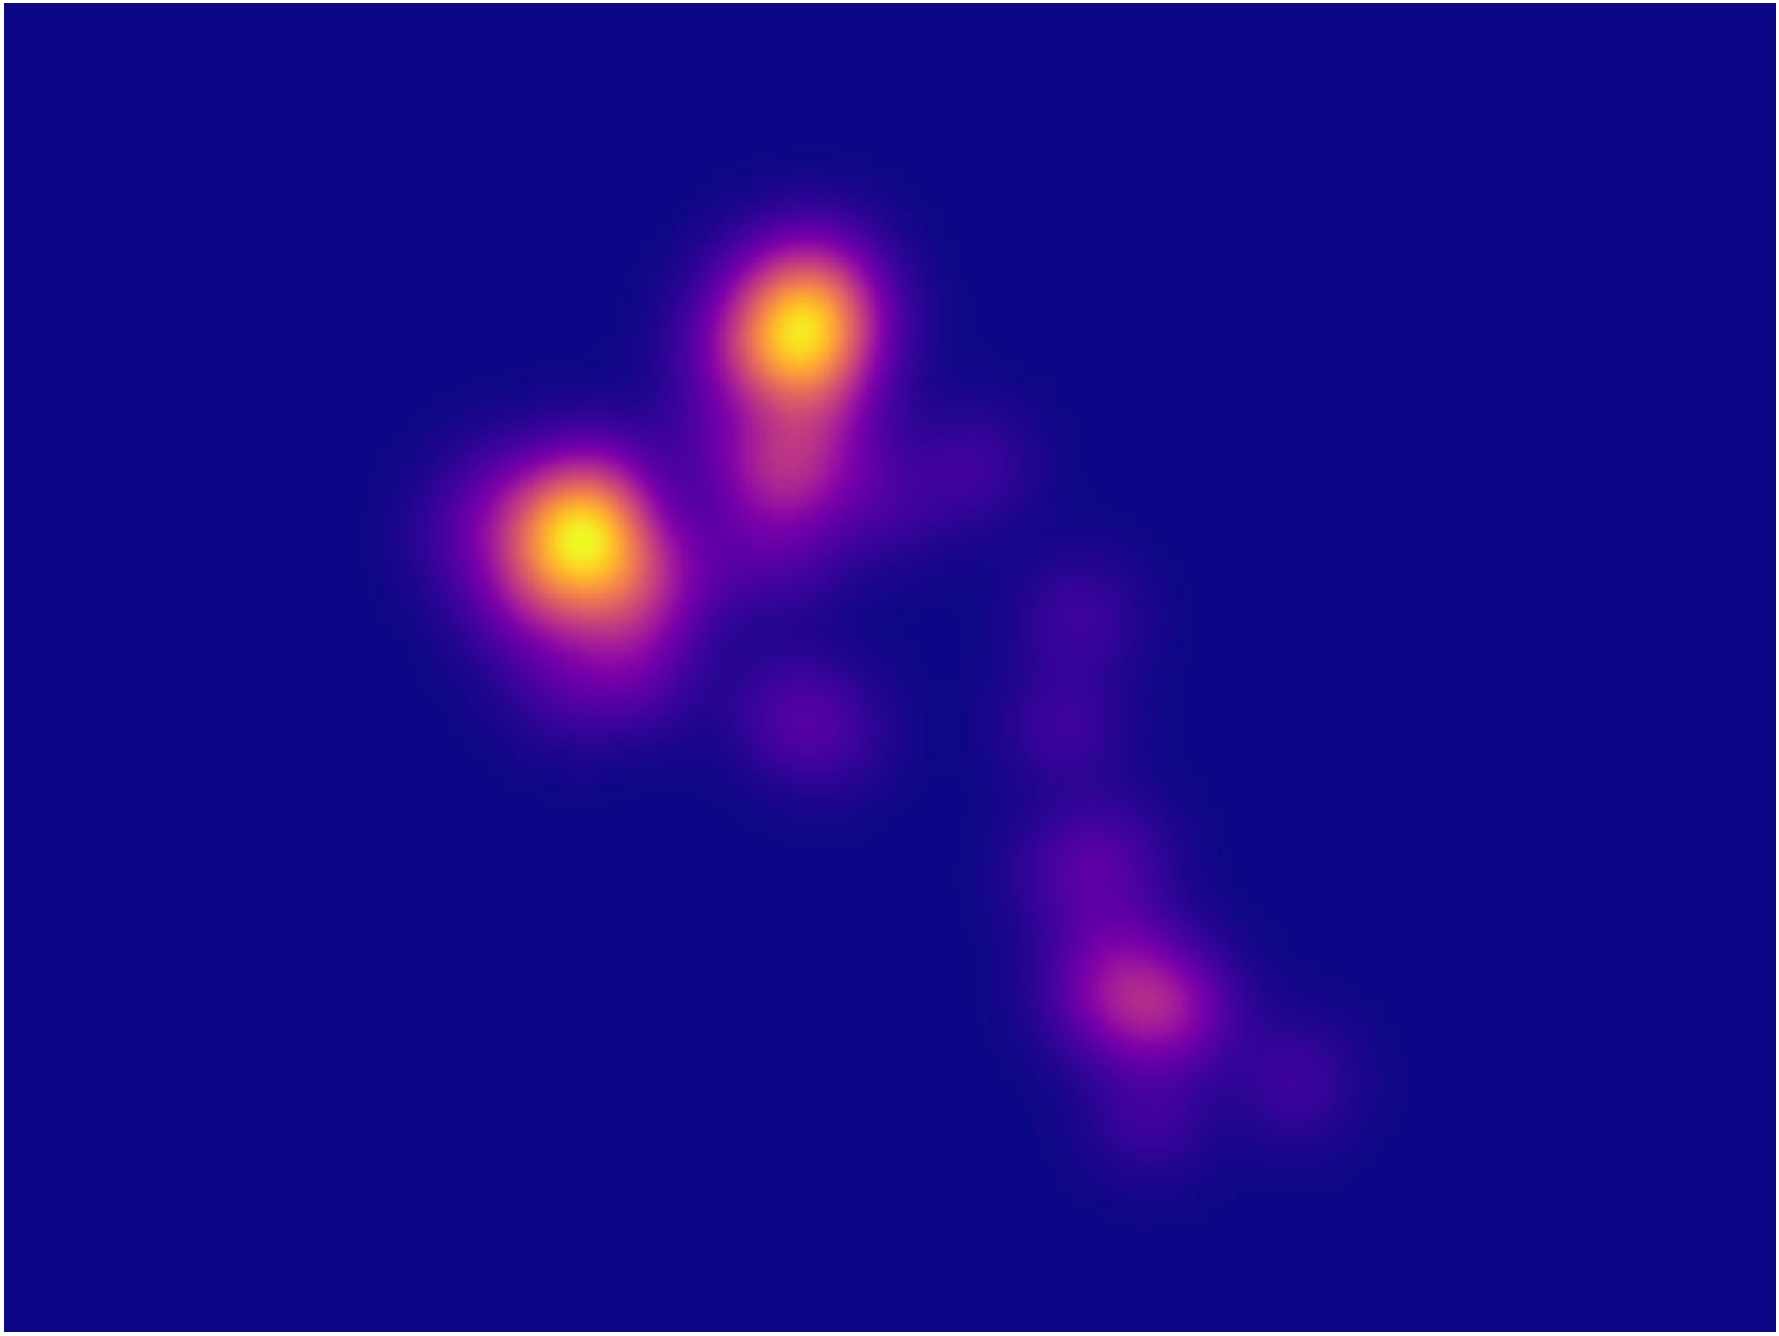
\includegraphics[width=0.25\textwidth]{./img/sign_gt.jpg} &
    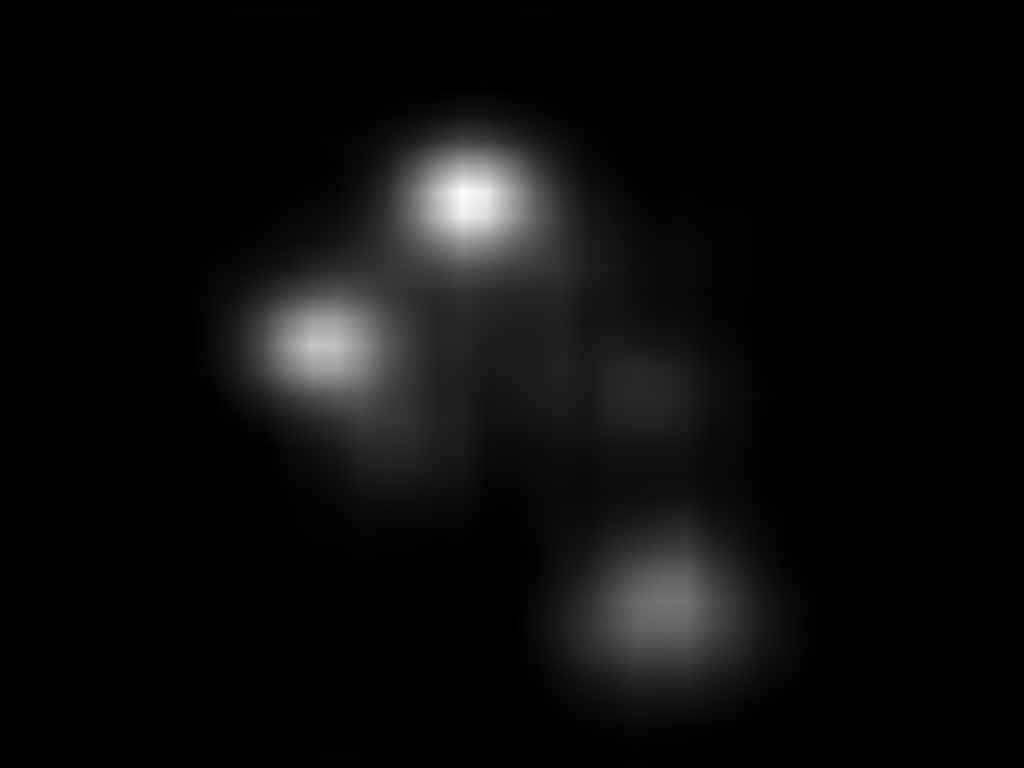
\includegraphics[width=0.25\textwidth]{./img/sign_m.jpg}\\
    \end{tabular}
\end{center}
    \caption{Examples of predictions made by the proposed model.}
    \label{fig:preds}
\end{figure*}

\section{Model evaluation}
\label{sec:metrics}
In order to assess how the maps generated by a model are similar to those
generated by humans, a variety of metrics has been used in the
literature~\cite{judd_2016}.
Some of the most used metrics are:
\begin{itemize}
    \item \emph{Area Under ROC Curve (AUC)}.
    Area under curve of true positive rate and false positive rate which is
    calculated from the binarized saliency map and the fixation points
    from human data for different thresholds.

    \item \emph{NSS}.
    Defined as:
	$$NSS(P, Q) = \frac{1}{N}\sum\limits_{i=1}^N{\bar{P_{i}}Q_{i}}$$
    Where $N$ is the number of fixation points in ground truth,
    $Q$ is the binary fixation points ground truth and $\bar{P}$ is the
    saliency map normalized by the standard deviation.
    NSS tends to penalize more false positives than AUC.

    \item \emph{Similarity}.
    Defined as:
	$$SIM(P, Q) = \frac{1}{N}\sum\limits_{i=1}^N{min(P_i, Q_i)}$$
    Where $P$ and $Q$ are both continuous saliency maps normalized
    by their sum.

    \item \emph{Cross-Correlation (CC)}.
    Defined as:
	$$CC(P, Q) = \frac{cov(P,Q)}{\sigma(P)\sigma(Q)}$$
    Where $P$ and $Q$ are both continuous saliency maps in $[0, 1]$.
    Similarity tends to penalize false negatives more than false positives.
    CC tends to penalize errors more symmetrically.
\end{itemize}

Visual saliency detection models are usually evaluated and ranked on
\emph{MIT saliency benchmark}~\cite{mit_sal_bm}, which uses the metrics
mentioned above -- in addition to a variety of others metrics --
to express how close generated saliency maps are to those created
from human data.
The most used dataset is \emph{MIT300},
which contains $300$ images of a variety of scenes and situations.
The ground truth data of \emph{MIT300} is held out.

\section{Results}
Prediction took an average time of 8 milliseconds.
Figure~\ref{fig:preds} shows some maps generated by the proposed model.

\subsection{Evaluation on the MIT300 benchmark}
Table~\ref{table:results} shows the resulting values for the most common
metrics on \emph{MIT300 benchmark}.
The proposed model achieved results comparable to those of the state of
the art while having, at least, one-fourth of the number of parameters.

\begin{table*}
	\small
    \begin{center}
    \label{table:results}
    \caption{State of the art models and metric scores on
    \emph{MIT300 benchmark}.}
    \begin{tabular}{|c|c|c|c|c|c|c|}
        \hline
        Model & Num. parameters & AUC-Judd $\uparrow$ & CC $\uparrow$
            & NSS $\uparrow$ & Sim $\uparrow$ & EMD $\downarrow$\\
        \hline
        Baseline: Infinite humans & - & 0.92 & 1.0 & 3.29 & 1.0 & 0\\
        \hline
        \emph{DeepFix} & $\approx$16.7 million & 0.87 & 0.78
            & 2.26 & 0.67 & 2.04\\
        \hline
        \emph{Salicon} & $\approx$14.7 million & 0.87 & 0.74 & 2.12
            & 0.60 & 2.62\\
        \hline
        \textbf{Proposed Model} & $\approx$\textbf{3.7 million}
            & \textbf{0.85} &
        \textbf{0.71} & \textbf{1.98} & \textbf{0.62} & \textbf{2.37}\\
        \hline
        \emph{ML-Net} & $\approx$15.4 million & 0.85 & 0.69 & 2.07 & 0.60
            & 2.53\\
        \hline
        \emph{SalNet} & $\approx$25.8 million & 0.83 & 0.57 & 1.51
            & 0.52 & 3.31\\
        \hline
    \end{tabular}
    \end{center}
\end{table*}

\section{Conclusion}
In this paper, we proposed a novel fully convolutional neural network for the
prediction of visual saliency on images.
The proposed model architecture was designed specifically
for the task of saliency prediction, with data pre-processing methods
specific for the context of saliency prediction.
Our methods showed to be effective, yielding to a network with performance
on \emph{MIT300 benchmark} consistently among the ten best results on various
metrics while having around $3/4$  fewer parameters than another state of
the art models.

{\small
\bibliographystyle{ieee}
\bibliography{bibliography}
}

\end{document}
